\documentclass{article}

% NeurIPS 2026 style (submission/default track)
\usepackage{neurips_2026}

\usepackage[utf8]{inputenc}
\usepackage[T1]{fontenc}
\usepackage{hyperref}
\usepackage{url}
\usepackage{booktabs}
\usepackage{amsfonts}
\usepackage{microtype}
\usepackage{xcolor}
\usepackage{amsmath, amssymb, amsthm}
\usepackage{graphicx}
\usepackage{algorithm}
\usepackage{algorithmic}
\usepackage{multirow}
\usepackage{subcaption}

\newtheorem{proposition}{Proposition}
\newtheorem{remark}{Remark}

\title{InteraSkill: Learning Reusable Skill Abstractions for Computer-Using Agents from Interaction Trajectories}
\author{Anonymous Authors}

\begin{document}

\maketitle

\begin{abstract}
Computer-using agents typically rely on manually engineered skill libraries---hard-coded mappings from semantic intents to fixed UI actions---that are brittle under interface changes and costly to maintain. We introduce \textsc{InteraSkill}, a three-phase framework that replaces manual skill specification with data-driven skill discovery, embedding, and composition. In Phase~1, trajectory segmentation via action discontinuity detection achieves boundary recall of 0.805 (F1\,=\,0.534) on fabricated data and F1\,=\,0.851 on real WebArena trajectories. In Phase~2, contrastive skill embedding with InfoNCE improves clustering NMI from 0.531 (Wasserstein baseline) to 0.871. In Phase~3, a LoRA-fine-tuned Qwen3-8B achieves 85.0\% skill prediction accuracy on enterprise workflows---a $4\times$ gain over a Transformer baseline and $6\times$ over a hard-coded transition table. On Mind2Web end-to-end evaluation, our method achieves 35.5\% task completion rate versus 9.5\% for the zero-shot baseline, with cross-domain transfer retaining 27.0\%. A six-model comparison across three benchmarks reveals that fine-tuning on interaction-derived data is critical: the LoRA-adapted 8B model outperforms zero-shot 70B models on in-domain tasks. Our results demonstrate that meaningful skill abstractions emerge from trajectory data without manual engineering, and that LLM-based composition with reasoning traces is essential for handling the contextual complexity of real workflows.
\end{abstract}

%==============================================================================
\section{Introduction}
%==============================================================================

Computer-using agents (CUAs) automate digital workflows by executing sequences of primitive actions---clicking, typing, scrolling---over graphical user interfaces~\cite{yao2022webshop,deng2023mind2web,zhou2024webarena}. Despite rapid progress, most systems rely on manually engineered skill specifications: configuration files that hard-code mappings between semantic intents and low-level execution details such as screen coordinates and UI element selectors. We refer to this pervasive but rarely formalized paradigm as \texttt{SKILL.md}.

While effective in controlled settings, \texttt{SKILL.md} introduces three fundamental limitations:
\begin{enumerate}
    \item \textbf{Brittleness.} Minor UI changes---layout shifts, element renaming---invalidate predefined skills, causing silent failures.
    \item \textbf{Inflexibility.} Extending to new interaction patterns requires manual engineering, preventing autonomous behavior discovery.
    \item \textbf{Scalability.} Large-scale deployments require hundreds of hand-crafted skills per domain, with maintenance costs that grow with both the number of environments and their rate of change.
\end{enumerate}

We propose \textsc{InteraSkill}, a framework that replaces manual skill specification with automatic skill discovery from interaction trajectories. Our approach operates in three phases: (1)~\emph{trajectory segmentation} identifies skill boundaries via action-space discontinuities; (2)~\emph{contrastive skill embedding} learns a structured latent space where behaviorally similar segments cluster together; and (3)~\emph{LLM-based skill composition} fine-tunes a language model on multi-turn conversations with reasoning traces and failure recovery to predict skill sequences for complex tasks.

Our central claim is empirical: \emph{agents that discover and compose skills from interaction data outperform those relying on fixed skill specifications, particularly on diverse, multi-step workflows.} We evaluate this claim through controlled experiments on fabricated enterprise trajectories (InteraSkill Workflows, IW), real WebArena navigation traces, Mind2Web cross-domain web tasks, and BrowseComp+ trajectories. Key findings include:

\begin{itemize}
    \item Contrastive skill embedding improves clustering NMI from 0.531 to 0.871 over an unsupervised Wasserstein baseline, recovering semantically meaningful skill structure.
    \item A LoRA-fine-tuned Qwen3-8B achieves 85.0\% skill prediction accuracy on IW data---outperforming a hard-coded \texttt{SKILL.md} table (14.0\%), AWM-style learned transitions (33.4\%), and a Transformer baseline (34.9\%).
    \item On Mind2Web end-to-end evaluation, InteraSkill achieves 35.5\% task completion rate (TCR) versus 9.5\% zero-shot, with cross-domain transfer retaining 76\% of in-domain performance (27.0\% TCR).
    \item A six-model comparison reveals that interaction-derived fine-tuning is critical: the LoRA-adapted 8B model outperforms zero-shot models up to 9$\times$ larger on in-domain tasks.
\end{itemize}

%==============================================================================
\section{Related Work}
%==============================================================================

\subsection{GUI Agents and the \texttt{SKILL.md} Paradigm}

Modern CUAs operate over structured UI representations with manually designed action spaces. WebShop~\cite{yao2022webshop} and Mind2Web~\cite{deng2023mind2web} established standard primitives (click, type, scroll), while WebArena~\cite{zhou2024webarena} and VisualWebArena~\cite{koh2024visualwebarena} provide realistic evaluation with 812 and 910 tasks respectively. Recent systems push performance substantially: OpAgent~\cite{guo2026opagent} achieves 71.6\% on WebArena via multi-agent architecture, OpenCUA~\cite{wang2025opencua} provides large-scale trajectory data (22.6K trajectories), and OSWorld~\cite{xie2024osworld} extends to full desktop environments. However, all assume predefined action primitives---the \texttt{SKILL.md} paradigm we seek to replace.

\subsection{Skill Discovery and Workflow Learning}

Several works address skill rigidity from different angles. Agent Workflow Memory (AWM)~\cite{wang2024awm} induces reusable workflow routines from trajectories, improving WebArena success by 51.1\% relative. SkillWeaver~\cite{zheng2025skillweaver} enables autonomous skill discovery through self-exploration, achieving 31.8\% WebArena improvement. AutoManual~\cite{chen2024automanual} constructs instruction manuals via agent exploration. ICAL~\cite{sarch2024ical} distills demonstrations and feedback into cognitive abstractions. LearnAct~\cite{liu2025learnact} shows that even a single demonstration improves performance by 198.9\% on mobile GUI tasks.

A critical gap remains (Table~\ref{tab:gap}): no existing work combines (1)~online skill discovery, (2)~learning from interaction trajectories rather than manual engineering, (3)~producing transferable skill abstractions, and (4)~continuous improvement. AWM mines workflows via LLM induction but not from grounded interaction patterns. SkillWeaver discovers skills autonomously but through self-exploration, not user-facing traces. ICAL produces per-instance memories rather than transferable abstractions. InteraSkill bridges this gap by learning reusable, composable skills directly from interaction data.

\begin{table}[t]
\centering
\caption{Comparison of skill acquisition approaches. InteraSkill is the first to combine all four desiderata: online operation, interaction-derived learning, transferable skill representations, and continuous self-improvement.}
\label{tab:gap}
\small
\begin{tabular}{lcccc}
\toprule
\textbf{Approach} & \textbf{Skill Source} & \textbf{Online} & \textbf{Interaction-Derived} & \textbf{Transferable} \\
\midrule
\texttt{SKILL.md} (manual) & Human engineering & \texttimes & \texttimes & \texttimes \\
AWM \cite{wang2024awm} & Trajectory mining & Partial & \texttimes & \checkmark \\
SkillWeaver \cite{zheng2025skillweaver} & Self-exploration & \texttimes & \texttimes & \checkmark \\
AutoManual \cite{chen2024automanual} & Agent exploration & \texttimes & \texttimes & \checkmark \\
ICAL \cite{sarch2024ical} & Demos + feedback & \checkmark & Partial & \texttimes \\
\textbf{InteraSkill (ours)} & \textbf{Interaction trajectories} & \checkmark & \checkmark & \checkmark \\
\bottomrule
\end{tabular}
\end{table}

\subsection{Unsupervised Skill Discovery}

The options framework~\cite{sutton1999between} and option-critic architecture~\cite{bacon2017option} formalize hierarchical behavior learning. DIAYN~\cite{eysenbach2018diversity} discovers diverse skills by maximizing mutual information $I(z; s)$ between skills and states. DADS~\cite{sharma2020dads} extends this to dynamics-aware discovery. CIC~\cite{laskin2022cic} uses contrastive learning to scale skill discovery to high-dimensional observations.

However, existing methods typically operate in low-dimensional robotic control with predefined actions. Our contribution is two-fold: (1)~we extend skill discovery to high-dimensional GUI environments where both perception and action are complex, and (2)~we use \emph{trajectory-level} mutual information $I(z; \tau \mid s_0)$ rather than state-level $I(z; s)$, capturing the temporal structure critical for multi-step GUI skills such as ``fill form'' or ``navigate menu.''

%==============================================================================
\section{Problem Formulation}
\label{sec:formulation}
%==============================================================================

We model CUA interaction as a hierarchical Markov Decision Process:
\begin{equation}
\mathcal{M} = (\mathcal{S}, \mathcal{A}_{\text{low}}, \mathcal{A}_{\text{high}}, P, R, \gamma),
\end{equation}
where $\mathcal{S} \subset \mathbb{R}^{h \times w \times 3}$ is the visual observation space, $\mathcal{A}_{\text{low}} = [0,1]^4$ is the continuous primitive action space, $\mathcal{A}_{\text{high}} = \mathcal{Z}$ is a learned latent skill space, $P$ is the transition dynamics, $R$ is the reward, and $\gamma$ is the discount factor.

The high-level controller selects a skill $z_t \sim \pi_H(\cdot \mid s_t)$ every $H$ low-level steps, while the low-level controller executes primitive actions $a_t \sim \pi_L(\cdot \mid s_t, z_{\lfloor t/H \rfloor})$. The objective is a bilevel optimization:
\begin{equation}
\max_{\pi_H, \pi_L} \; \mathbb{E}\left[\sum_{t=0}^{T} \gamma^t R(s_t, a_t)\right], \quad \text{s.t.} \quad z_t \sim \pi_H(\cdot \mid s_t), \quad a_t \sim \pi_L(\cdot \mid s_t, z_t).
\end{equation}

The key insight is that $\mathcal{A}_{\text{high}}$ need not be manually specified. We learn $\mathcal{Z}$ from data, such that each $z \in \mathcal{Z}$ corresponds to a semantically meaningful, reusable behavior pattern. This eliminates \texttt{SKILL.md} by making skill abstractions emergent rather than engineered.

%==============================================================================
\section{Method: The InteraSkill Framework}
\label{sec:method}
%==============================================================================

\subsection{Phase 1: Trajectory Segmentation}

Given raw action trajectories, we identify skill boundaries via action discontinuities. For a trajectory $(a_0, a_1, \ldots, a_T)$, we compute:
\begin{equation}
\Delta a_t = \|a_t - a_{t-1}\|_2, \quad t \in \mathcal{B} \;\text{if}\; \Delta a_t > \theta,
\end{equation}
where $\theta$ is a threshold selected by sweeping percentiles of the action-difference distribution. Boundary points $\mathcal{B}$ partition each trajectory into candidate skill segments. The intuition is that significant changes in action pattern signal transitions between distinct behaviors (e.g., from navigating to typing).

\subsection{Phase 2: Skill Embedding}

\paragraph{Step 1: Segment Representation.}
Each segment is modeled as a Gaussian mixture over its constituent actions:
\begin{equation}
p(a \mid \text{segment}_i) = \sum_{m} \pi_m \mathcal{N}(a; \mu_m, \Sigma_m),
\end{equation}
capturing the action distribution within the segment independently of sequence length.

\paragraph{Step 2: Wasserstein Clustering.}
We group similar segments using an approximate distributional distance:
\begin{equation}
D(\text{seg}_i, \text{seg}_j) = \| \mu_i - \mu_j \|_2^2 + \| \Sigma_i - \Sigma_j \|_F^2,
\label{eq:bures}
\end{equation}
which corresponds to the squared Bures metric between Gaussians---an approximation to the 2-Wasserstein distance. Agglomerative clustering on this distance matrix discovers the natural number of skill types without manual specification. We use the resulting cluster assignments as pseudo-labels for contrastive learning.

\paragraph{Step 3: Contrastive Skill Embedding.}
We train a neural encoder $f_\theta$ to map trajectory segments into a $d$-dimensional latent space $\mathcal{Z} = \mathbb{R}^{d_{\text{skill}}}$, optimizing an InfoNCE objective~\cite{oord2018cpc}:
\begin{equation}
\mathcal{L}_{\text{skill}} = -\mathbb{E}_{\tau} \left[ \log \frac{\exp(f(\tau, z_\tau)/T)}{\sum_{z'} \exp(f(\tau, z')/T)} \right],
\label{eq:infonce}
\end{equation}
where $z_\tau$ is the cluster assignment (pseudo-label) of trajectory $\tau$, and $T$ is the temperature. This objective maximizes mutual information $I(z; \tau \mid s_0)$ between skills and trajectories: each skill learns to explain a distinct trajectory pattern while being discriminated from others.

\emph{Clarification on supervision.} Our approach is not fully unsupervised: Phase~2 uses pseudo-labels from the Wasserstein clustering (Step~2) as positive-pair anchors for the InfoNCE loss. The clustering itself is unsupervised, but the contrastive encoder leverages its output. This two-stage pipeline---unsupervised clustering followed by contrastive refinement---yields substantially better representations than either stage alone (Section~\ref{sec:results_discovery}).

\subsection{Phase 3: Skill Composition}

Once skills are discovered and embedded, we train models to compose them for complex tasks. We evaluate three approaches of increasing capacity:

\paragraph{MLP Baseline.} An MLP takes the current skill embedding concatenated with a position scalar and predicts the next skill. This tests whether local skill context suffices for composition.

\paragraph{Transformer Decoder.} A 2-layer causal Transformer ($d_{\text{model}}=64$, 4 heads) attends over the full skill sequence, testing whether sequential context improves composition.

\paragraph{LLM with LoRA.} We fine-tune Qwen3-8B using QLoRA (4-bit quantization, rank-16 adapters on attention projections, 0.2\% trainable parameters) on 1,275 multi-turn user-agent conversations. These conversations include: (i)~reasoning traces with explicit skill selection rationale, (ii)~user corrections requiring mid-workflow adaptation, and (iii)~failure recovery scenarios spanning API timeouts, permission errors, and cascading failures. This tests whether world knowledge and contextual reasoning improve composition beyond pattern matching.

\paragraph{Options-Based Execution.}
Each discovered skill $z$ corresponds to a semi-Markov option with policy $\pi_z(a \mid s)$ and learned termination condition $\beta_z(s) \in [0,1]$. The option-value recursion is:
\begin{equation}
Q(s, z) = r(s, z) + \gamma \mathbb{E}_{s'} \left[ (1 - \beta_z(s')) Q(s', z) + \beta_z(s') \max_{z'} Q(s', z') \right],
\end{equation}
enabling dynamic skill switching based on state feedback rather than fixed sequences.

\subsection{Cross-Domain Transfer}

Skills transfer across domains when their semantic meaning is preserved despite visual differences. We quantify transferability via:
\begin{equation}
\text{Inv}(z_A, z_B) = \mathbb{E}_{s_A, s_B} \left[\text{KL}(\pi_{z_A}(\cdot \mid s_A) \,\|\, \pi_{z_B}(\cdot \mid s_B))\right],
\end{equation}
where states are matched semantically using CLIP embeddings: $\text{Sim}(s_A, s_B) = \cos(\phi_{\text{CLIP}}(s_A), \phi_{\text{CLIP}}(s_B))$. Low invariance indicates skills that generalize across visual domains. We evaluate cross-domain transfer empirically in Section~\ref{sec:results_e2e} rather than relying on theoretical bounds, as the assumptions required for formal guarantees (shared semantic state spaces, bounded domain shift) are difficult to verify in practice.

%==============================================================================
\section{Experimental Setup}
\label{sec:setup}
%==============================================================================

\subsection{Datasets}

We evaluate on four datasets spanning synthetic and real-world GUI interactions:

\paragraph{InteraSkill Workflows (IW).} 500 fabricated interaction trajectories spanning 12 skill types (e.g., \texttt{document\_edit}, \texttt{search\_navigate}, \texttt{send\_message}), totaling 2,108 ground-truth segments. These trajectories simulate enterprise workflows including document editing, communication, and file management. Ground-truth skill labels enable controlled evaluation of the discovery pipeline.

\paragraph{Mind2Web~\cite{deng2023mind2web}.} A large-scale dataset of real web interaction traces across 137 websites in 31 domains. We evaluate on both the \emph{test\_task} split (tasks from seen domains) and \emph{test\_domain} split (tasks from entirely unseen domains) to measure cross-domain generalization. Each trajectory includes HTML snapshots, action annotations, and natural language task descriptions.

\paragraph{WebArena~\cite{zhou2024webarena}.} 1,000 real navigation trajectories from the map domain, providing 3,140 segments. This dataset tests the pipeline on realistic, repetitive web interactions with limited skill diversity.

\paragraph{BrowseComp+.} Trajectories derived from the BrowseComp benchmark, testing generalization to complex browsing tasks with diverse action patterns.

\subsection{Models Compared}

For Phase~3 skill composition, we evaluate six language models:
\begin{itemize}
    \item \textbf{Qwen3-8B} (zero-shot and LoRA-fine-tuned) --- our primary model
    \item \textbf{Llama-3.1-70B} (zero-shot) --- testing whether scale compensates for lack of fine-tuning
    \item \textbf{DeepSeek-R1-Distill-Qwen-32B} (zero-shot) --- reasoning-specialized model
    \item \textbf{Gemma-4-31B} (zero-shot) --- Google's open model
    \item \textbf{OLMo-3-7B} (zero-shot) --- fully open-source baseline
\end{itemize}

We also compare against structural baselines: a hard-coded \texttt{SKILL.md} transition table, AWM-style bigram transitions~\cite{wang2024awm}, and a most-frequent-skill predictor.

\subsection{Metrics}

\paragraph{Skill Discovery (Phases 1--2).} Boundary precision/recall/F1 for segmentation; Normalized Mutual Information (NMI), silhouette score, and purity for clustering quality.

\paragraph{Skill Composition (Phase 3).} Per-position accuracy, exact sequence match rate, and normalized edit distance for skill prediction.

\paragraph{End-to-End (Mind2Web).} Task Completion Rate (TCR): a task is complete when all predicted actions match ground-truth actions in sequence. Per-step action accuracy and element accuracy provide fine-grained diagnostics.

\subsection{Implementation Details}

\paragraph{Phase 1.} We sweep $\theta$ across percentiles of the $\Delta a_t$ distribution. Results are robust across the 40th--60th percentile range.

\paragraph{Phase 2.} The contrastive encoder is a 3-layer MLP ($d_{\text{input}} = 8 \to 64 \to 32 \to d_{\text{skill}} = 16$) with ReLU activations and batch normalization, trained for 200 epochs with Adam (lr=$10^{-3}$), batch size 128, temperature $T = 0.07$.

\paragraph{Phase 3 (LoRA).} Qwen3-8B fine-tuned with QLoRA: 4-bit NF4 quantization, rank 16, $\alpha = 16$, dropout 0.05, applied to $\{q, k, v, o\}_{\text{proj}}$. Training: 3 epochs, lr=$2 \times 10^{-4}$, batch size 4, gradient accumulation 4, cosine schedule. Total trainable parameters: 17M (0.2\% of 8B). Training time: 31 minutes on a single A6000.

\paragraph{Phase 3 (GRPO).} We also train Qwen3-8B with Group Relative Policy Optimization using a composite reward: $+1.0$ for correct skill prediction, $+0.3$ for correct action format, $+0.1$ for reasoning presence, $-0.3$ for unparseable output. GRPO generates 4 candidate responses per prompt at temperature 0.7, with LoRA rank 16 and cosine schedule (lr=$5 \times 10^{-5}$, warmup 10\%).

All experiments use NVIDIA A6000 GPUs (48GB). Phase~1--2 experiments run on a single GPU; Phase~3 LoRA training uses 1 GPU; GRPO uses 4 GPUs with a 3-day time limit.

%==============================================================================
\section{Results}
\label{sec:results}
%==============================================================================

\subsection{Phase 1: Trajectory Segmentation}

On IW data, sweeping $\theta$ across percentiles yields optimal performance at $\theta = 1.550$ (50th percentile): boundary precision 0.415, recall 0.805, F1 0.534 (Figure~\ref{fig:segmentation}). The high recall indicates that most true skill boundaries produce detectable action discontinuities. Precision is lower because some within-skill action variation exceeds the threshold---incorporating additional features (e.g., DOM state changes) could improve boundary detection.

On WebArena trajectories, segmentation quality is higher: the optimal threshold ($\theta = 0.603$) achieves F1 = 0.851. The improvement reflects WebArena's more structured action patterns compared to the diverse enterprise workflows in IW.

\begin{figure}[h]
\centering
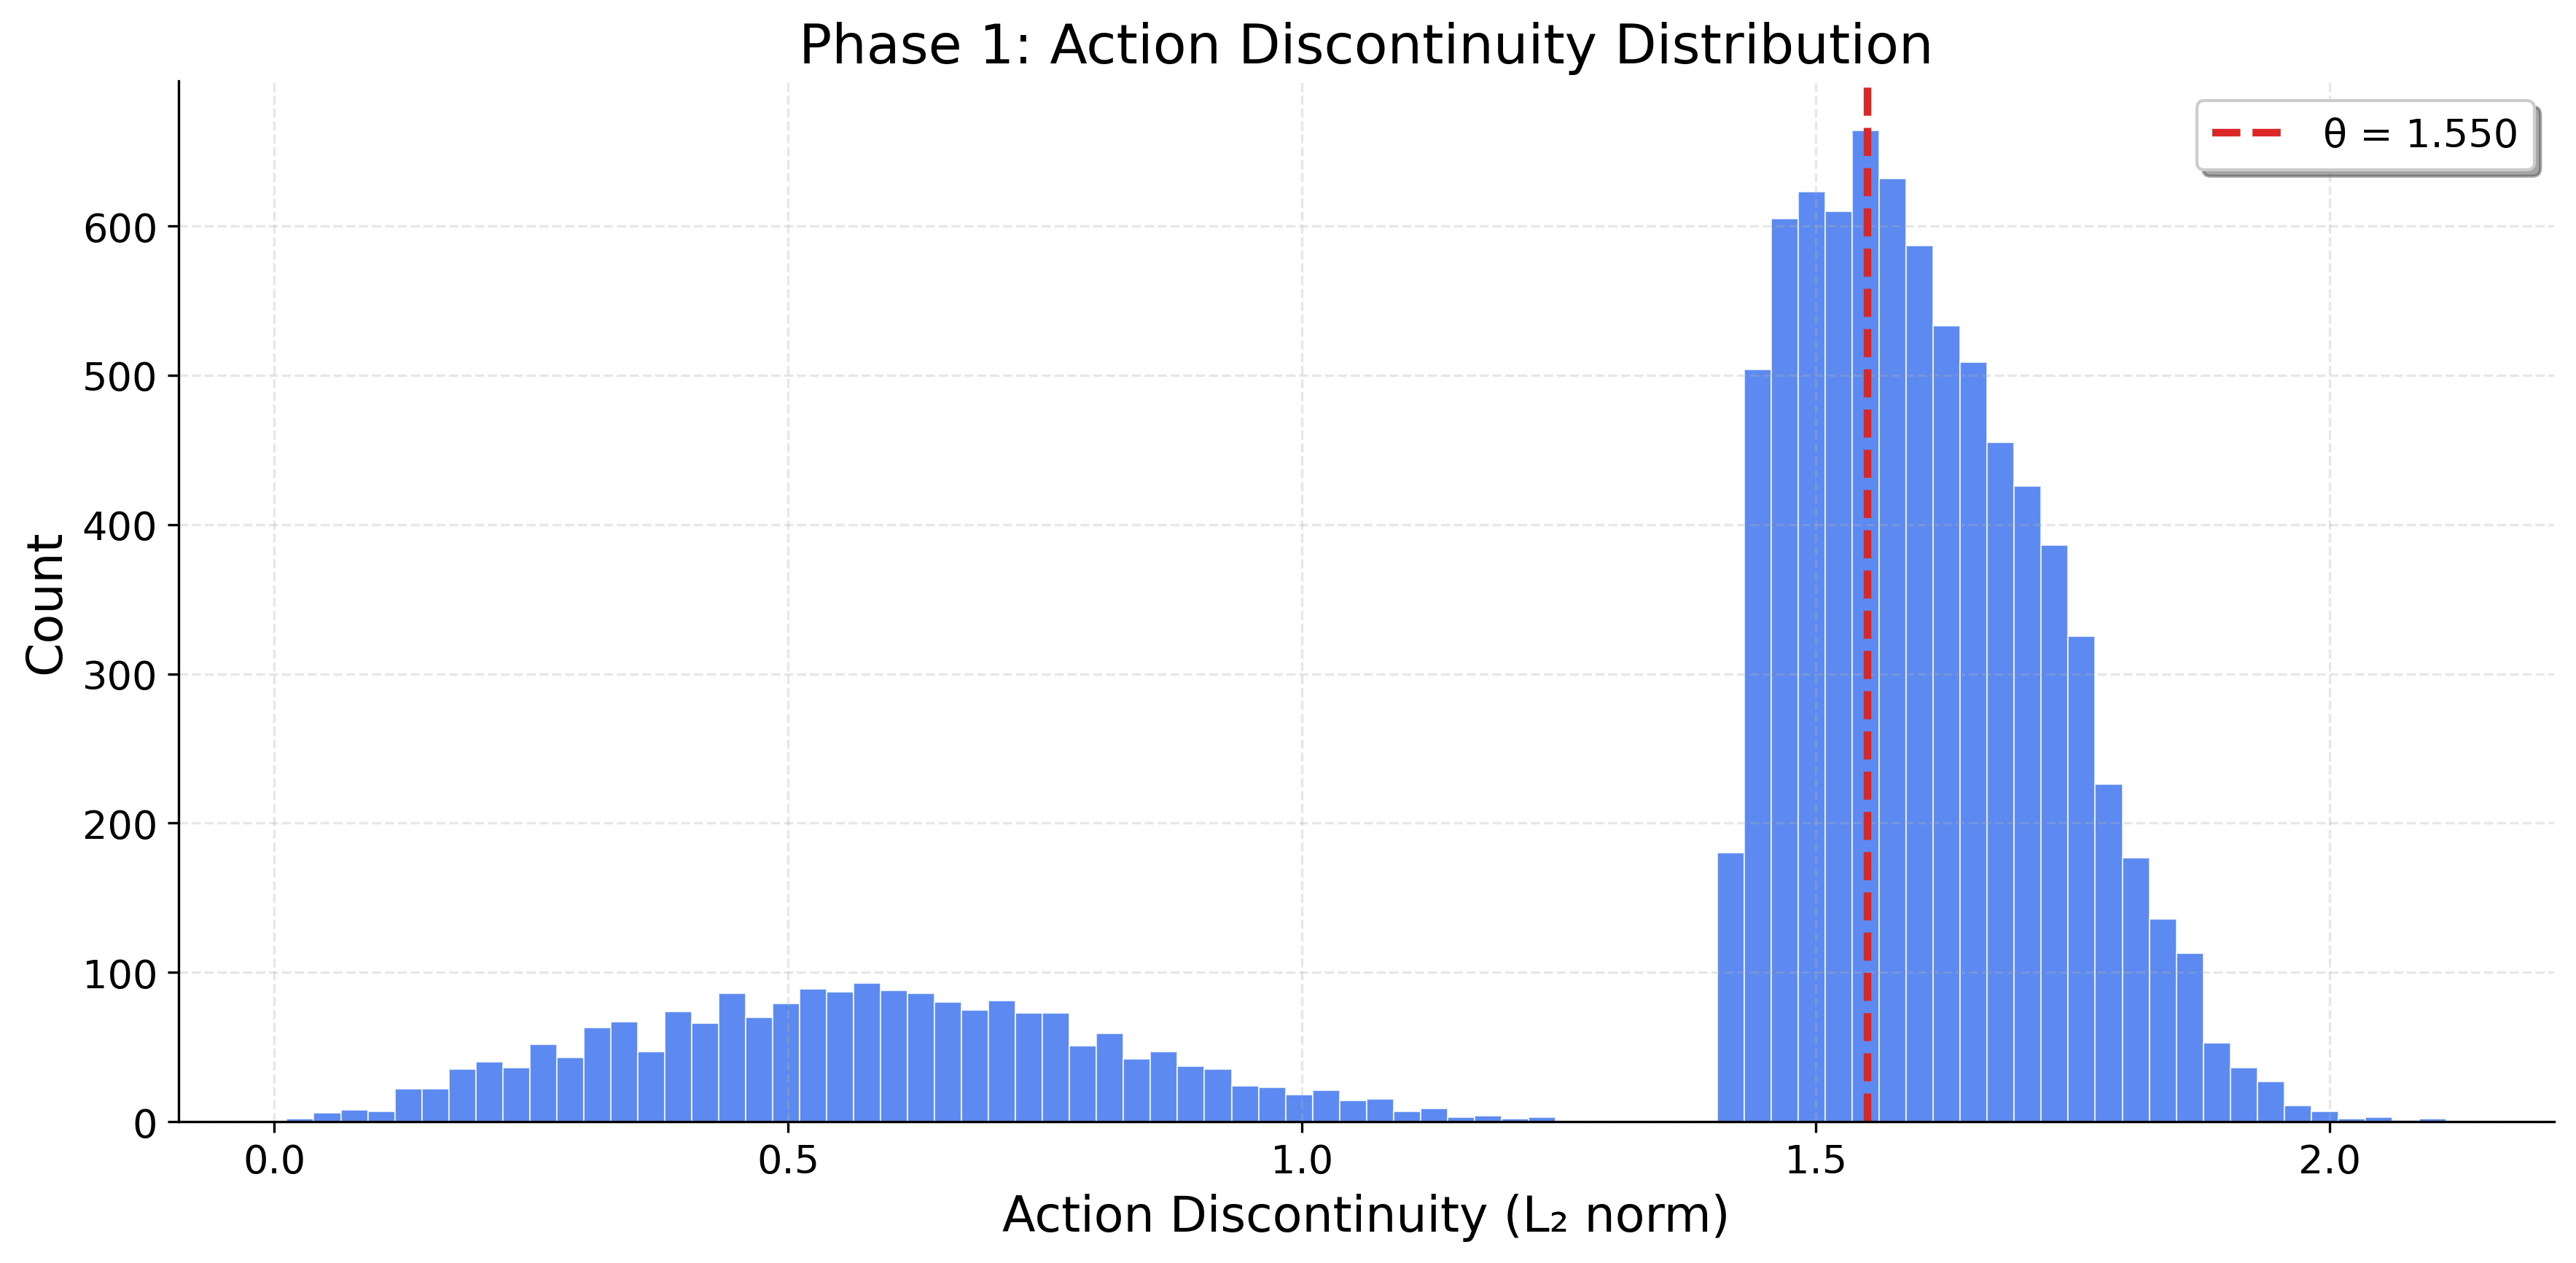
\includegraphics[width=0.85\textwidth]{../results/figures/segmentation_hist.png}
\caption{Distribution of action discontinuities ($\|\Delta a_t\|_2$) across all IW trajectories, with optimal threshold $\theta = 1.550$ (dashed line). Values above $\theta$ are classified as skill boundaries. The bimodal structure reflects within-skill variation (left peak) versus between-skill transitions (right peak).}
\label{fig:segmentation}
\end{figure}

\subsection{Phase 2: Skill Discovery and Embedding}
\label{sec:results_discovery}

\paragraph{Wasserstein Clustering.}
Using the Bures metric (Eq.~\ref{eq:bures}), agglomerative clustering achieves NMI = 0.531 at $k = 10$ on IW data (Table~\ref{tab:clustering}). NMI is stable across $k \in \{8, 10, 12\}$, while purity increases monotonically with $k$---the expected behavior as over-segmentation trivially increases within-cluster homogeneity. We select $k = 10$ as a balance between NMI and purity.

\begin{table}[h]
\centering
\caption{Wasserstein clustering quality on IW data across different numbers of clusters $k$.}
\label{tab:clustering}
\small
\begin{tabular}{ccc}
\toprule
$k$ & NMI & Purity \\
\midrule
8  & 0.531 & 0.528 \\
10 & \textbf{0.531} & 0.528 \\
12 & 0.502 & 0.532 \\
14 & 0.508 & 0.581 \\
16 & 0.508 & 0.597 \\
\bottomrule
\end{tabular}
\end{table}

\paragraph{Contrastive Refinement.}
Training the InfoNCE encoder (Eq.~\ref{eq:infonce}) for 200 epochs using Wasserstein cluster assignments as pseudo-labels yields dramatically improved representations. In the learned 16-dimensional latent space, KMeans clustering achieves NMI = 0.871, silhouette = 0.561, purity = 0.869---a 64\% relative improvement in NMI over the Wasserstein baseline. The t-SNE visualization (Figure~\ref{fig:tsne}) confirms well-separated clusters corresponding to distinct skill types. Training curves (Figure~\ref{fig:training}) show smooth convergence with no overfitting.

On WebArena, segmentation quality is high (F1 = 0.851), but embedding quality is substantially lower (NMI = 0.049, silhouette = $-0.255$). The negative silhouette indicates overlapping clusters, reflecting the limited skill diversity in map-only navigation data. This highlights a fundamental limitation: contrastive skill embedding requires diverse behavioral patterns to learn discriminative representations.

\begin{figure}[h]
\centering
\begin{subfigure}[b]{0.48\textwidth}
    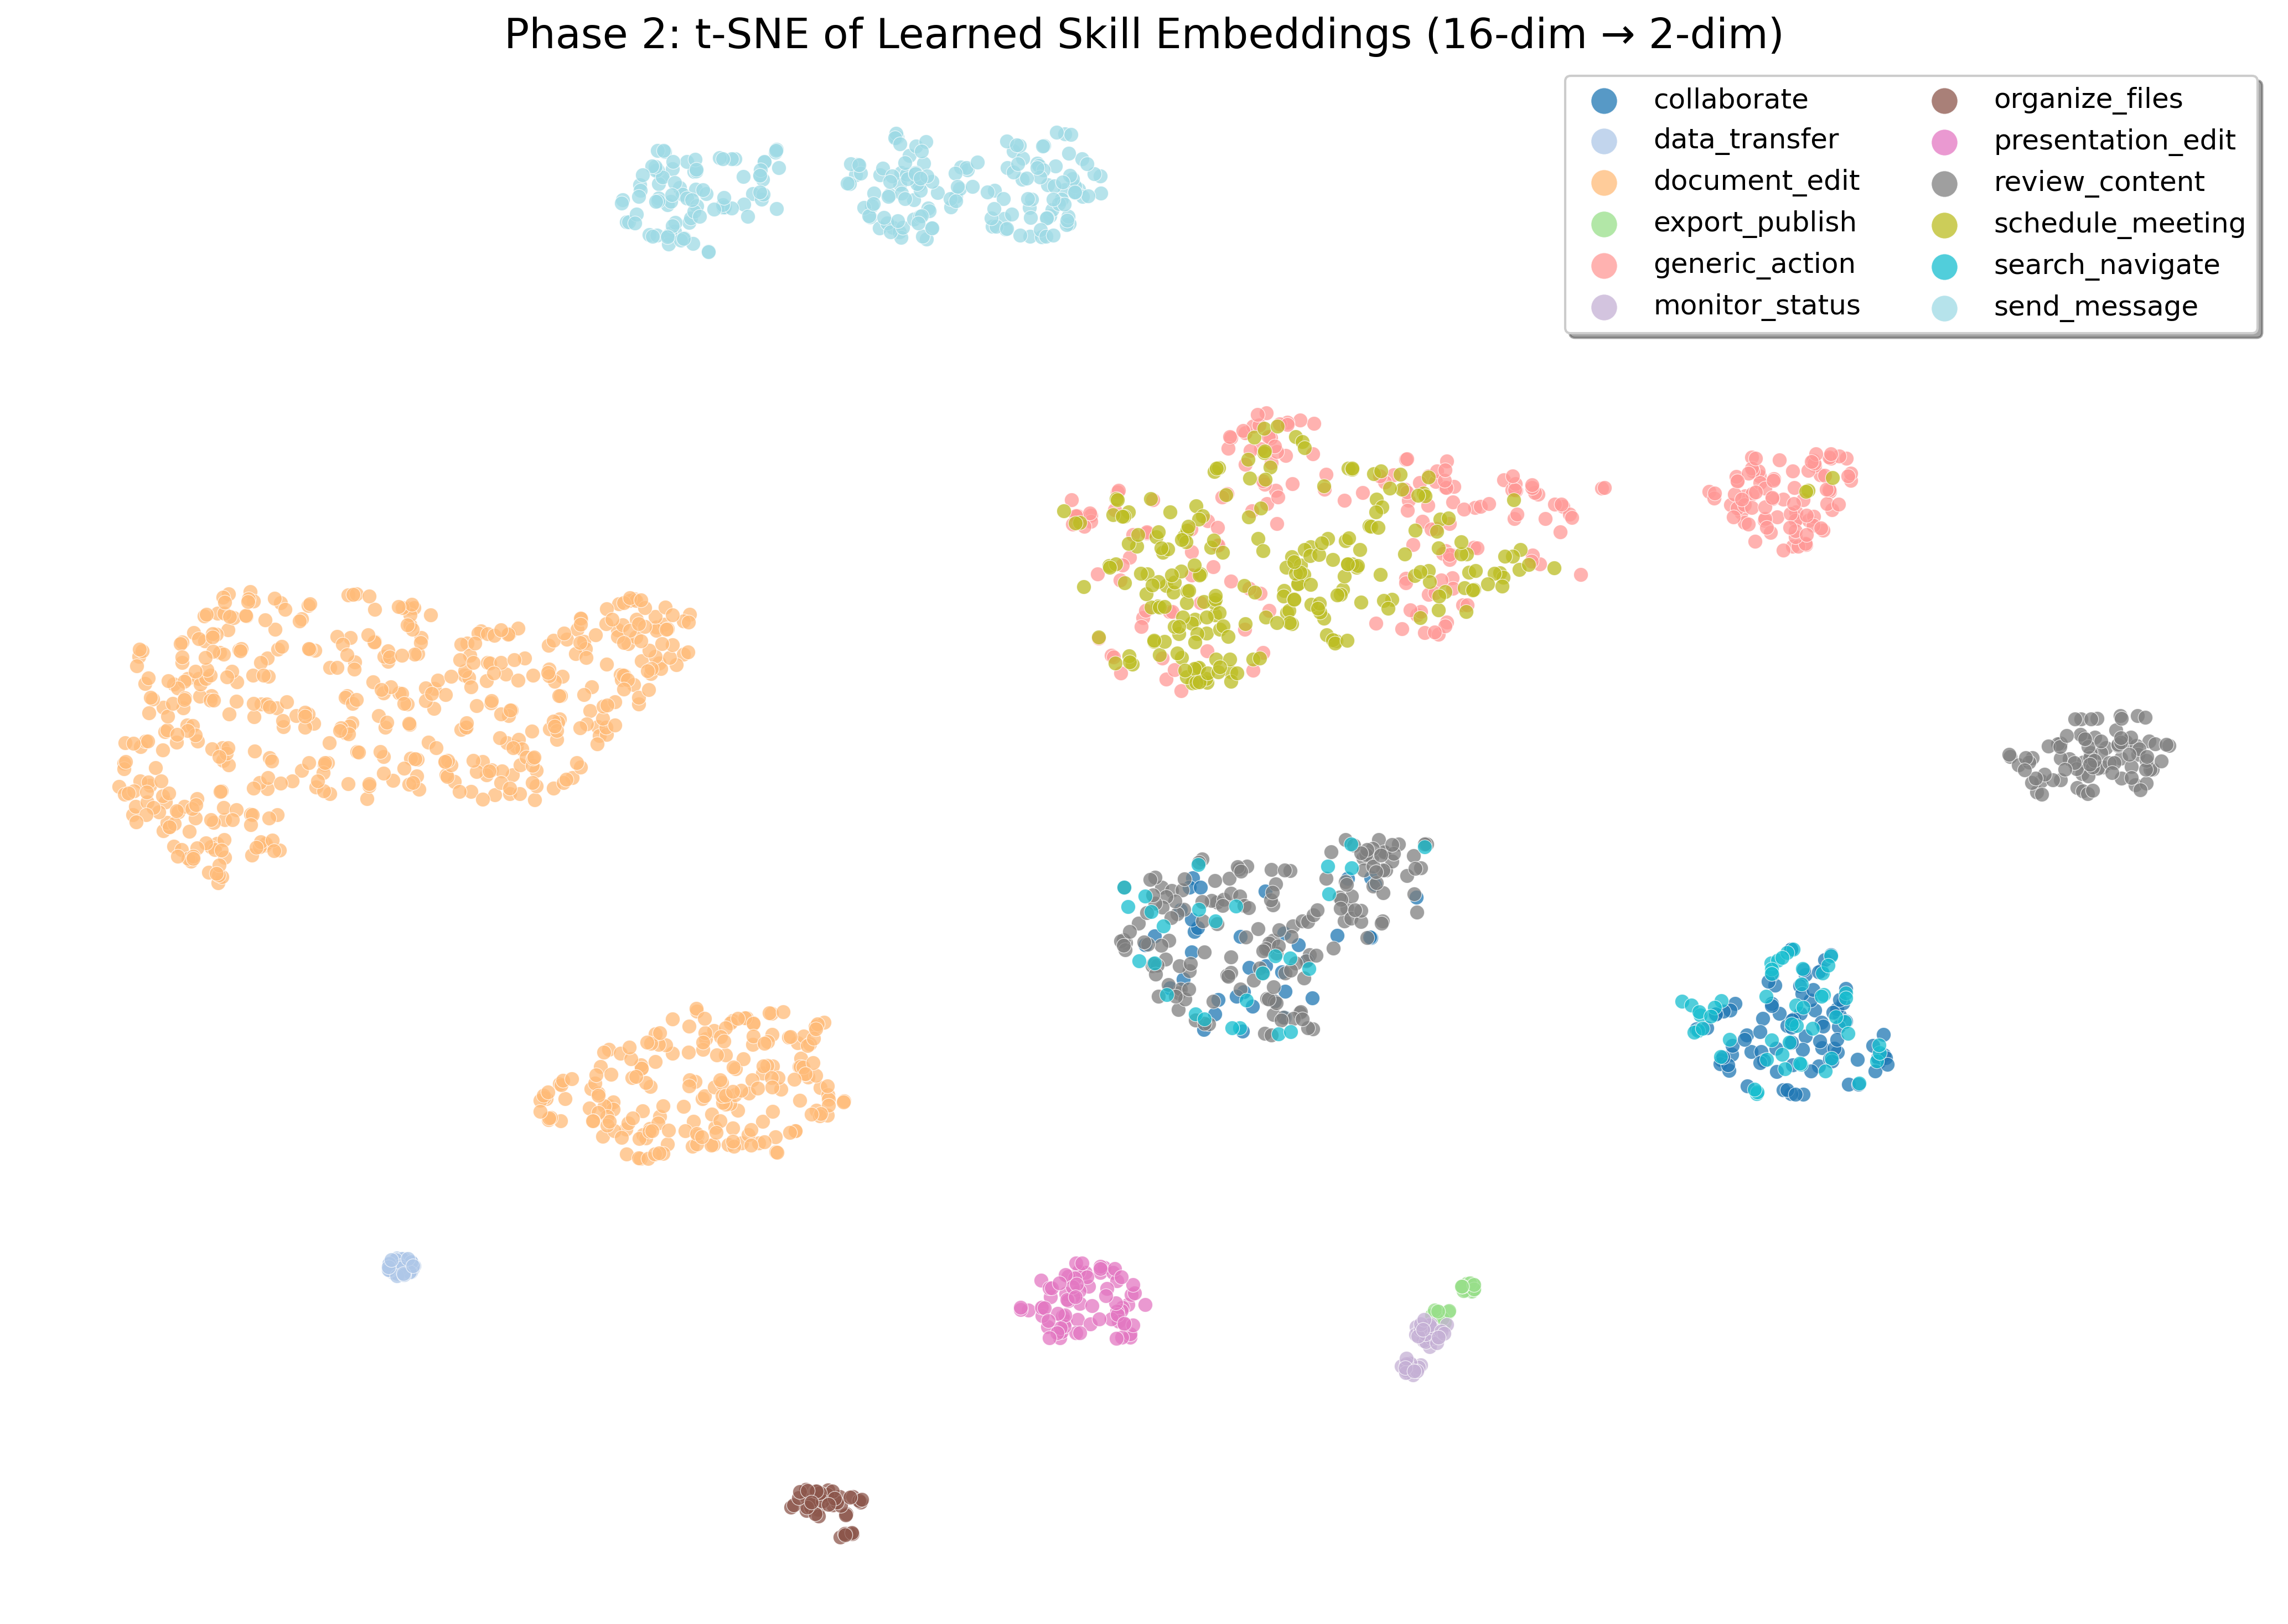
\includegraphics[width=\textwidth]{../results/figures/tsne.png}
    \caption{t-SNE of 16-dim skill embeddings on IW data. Colors indicate ground-truth skill types. Well-separated clusters confirm discriminative representation learning.}
    \label{fig:tsne}
\end{subfigure}
\hfill
\begin{subfigure}[b]{0.48\textwidth}
    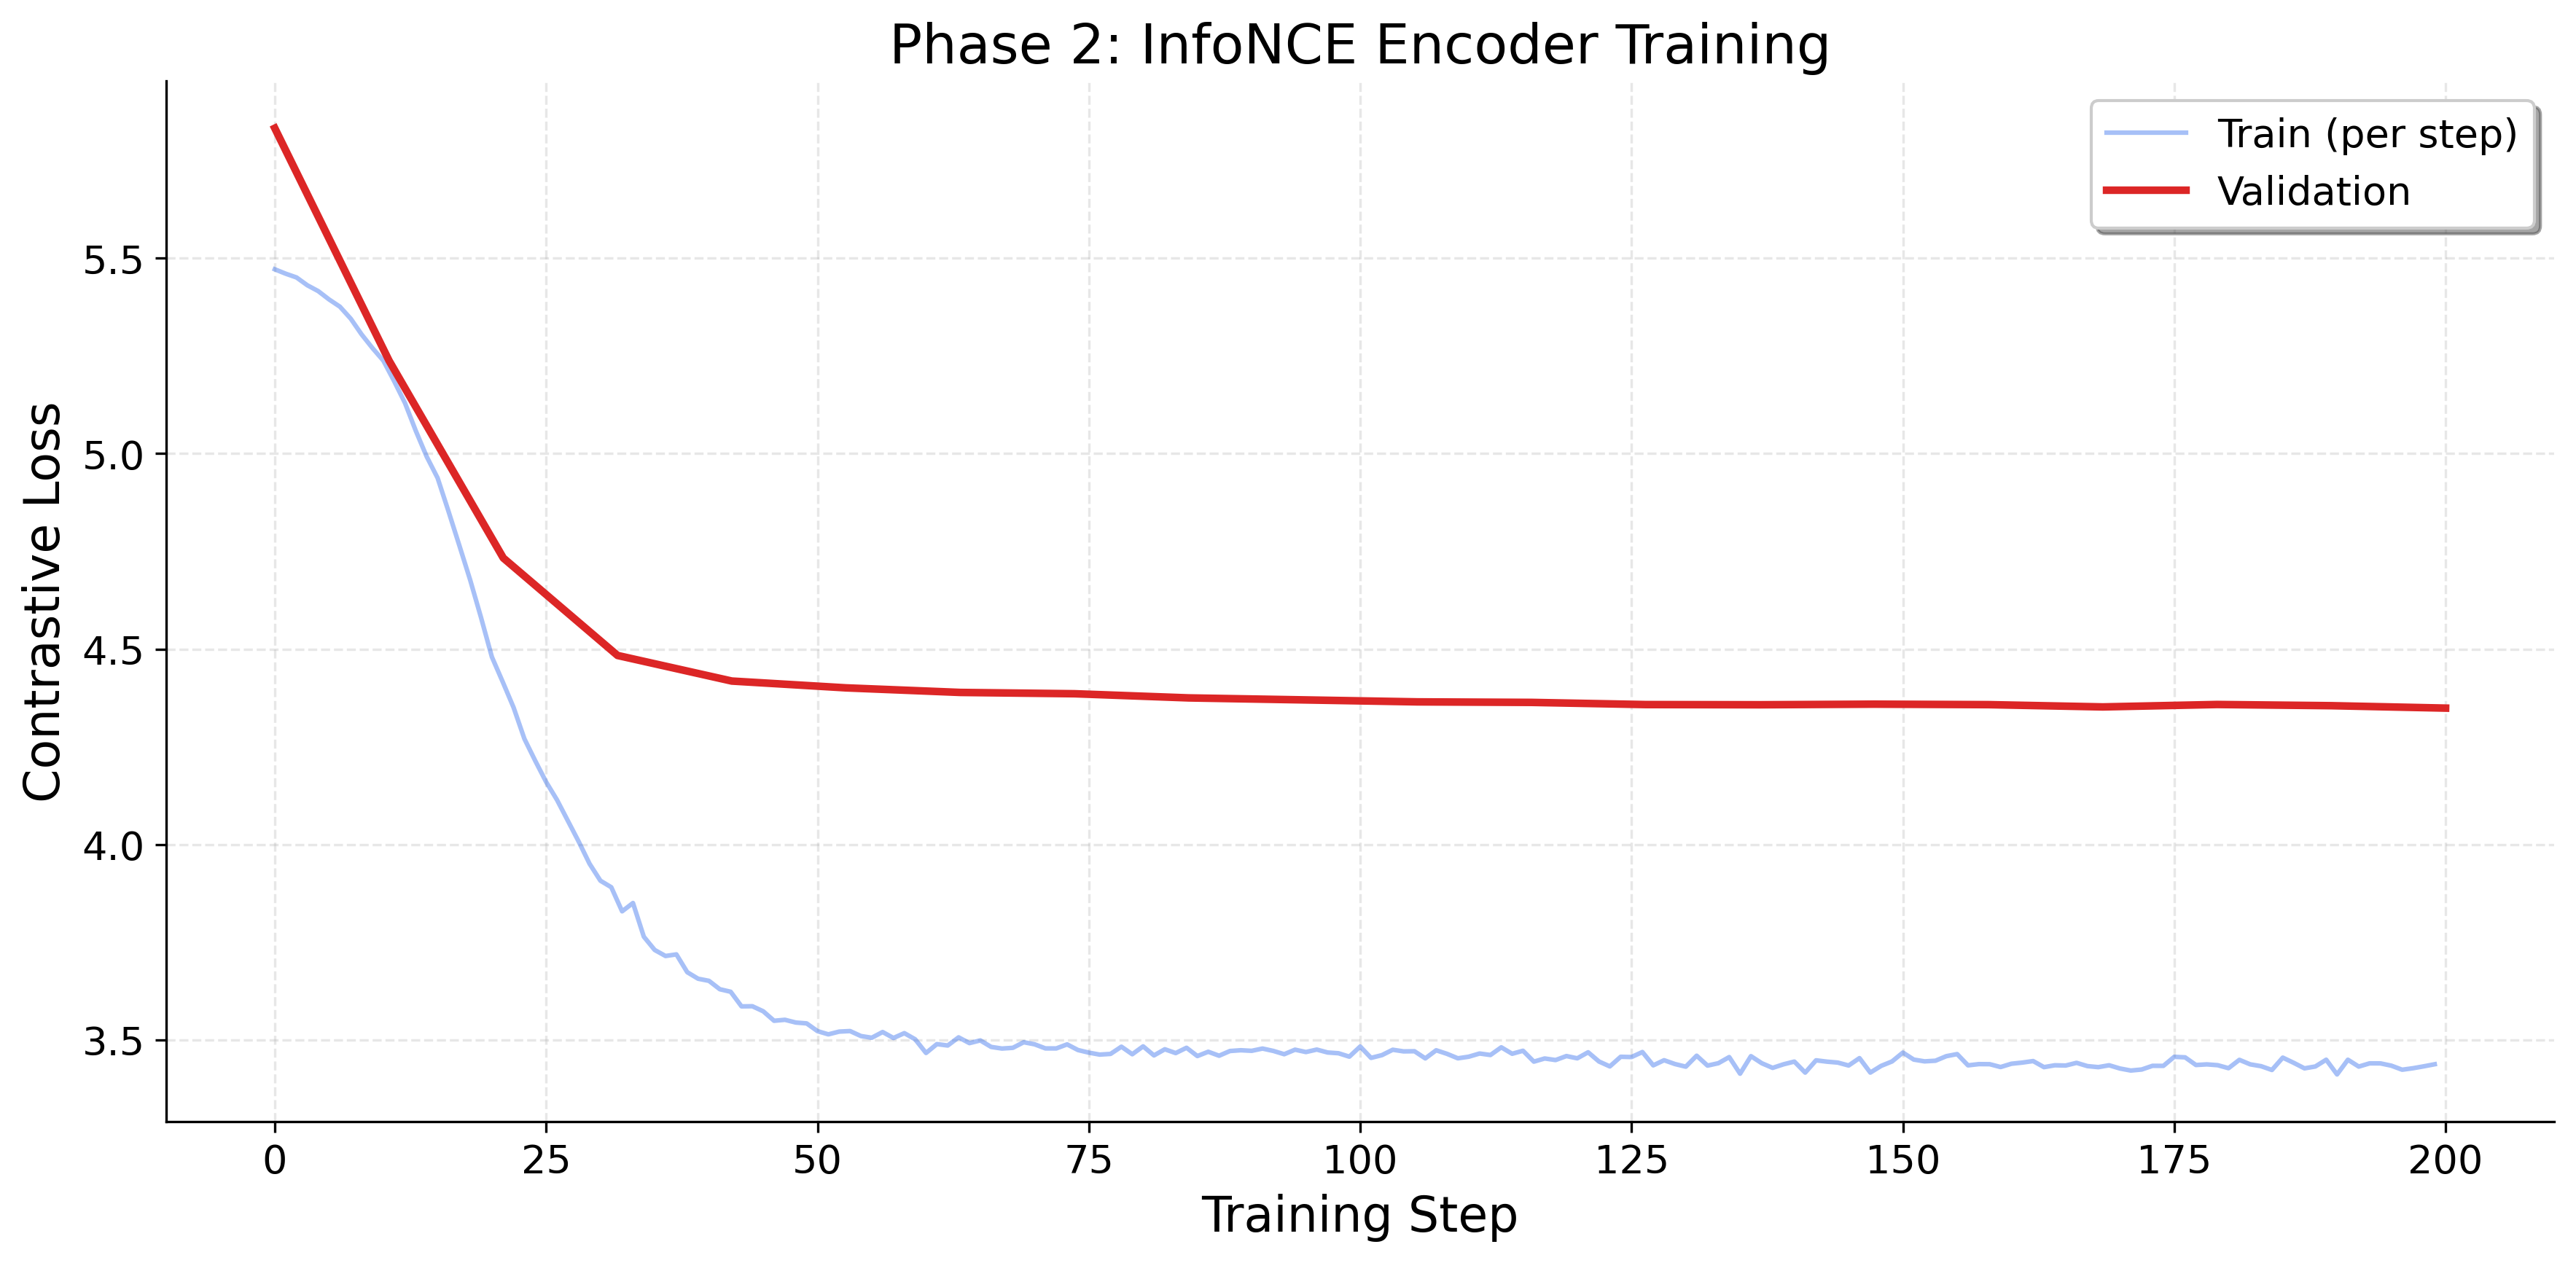
\includegraphics[width=\textwidth]{../results/figures/training_curves.png}
    \caption{InfoNCE training and validation loss over 200 epochs. Smooth convergence with stable validation loss indicates no overfitting.}
    \label{fig:training}
\end{subfigure}
\caption{Phase 2 skill embedding results on IW data.}
\end{figure}

\begin{figure}[h]
\centering
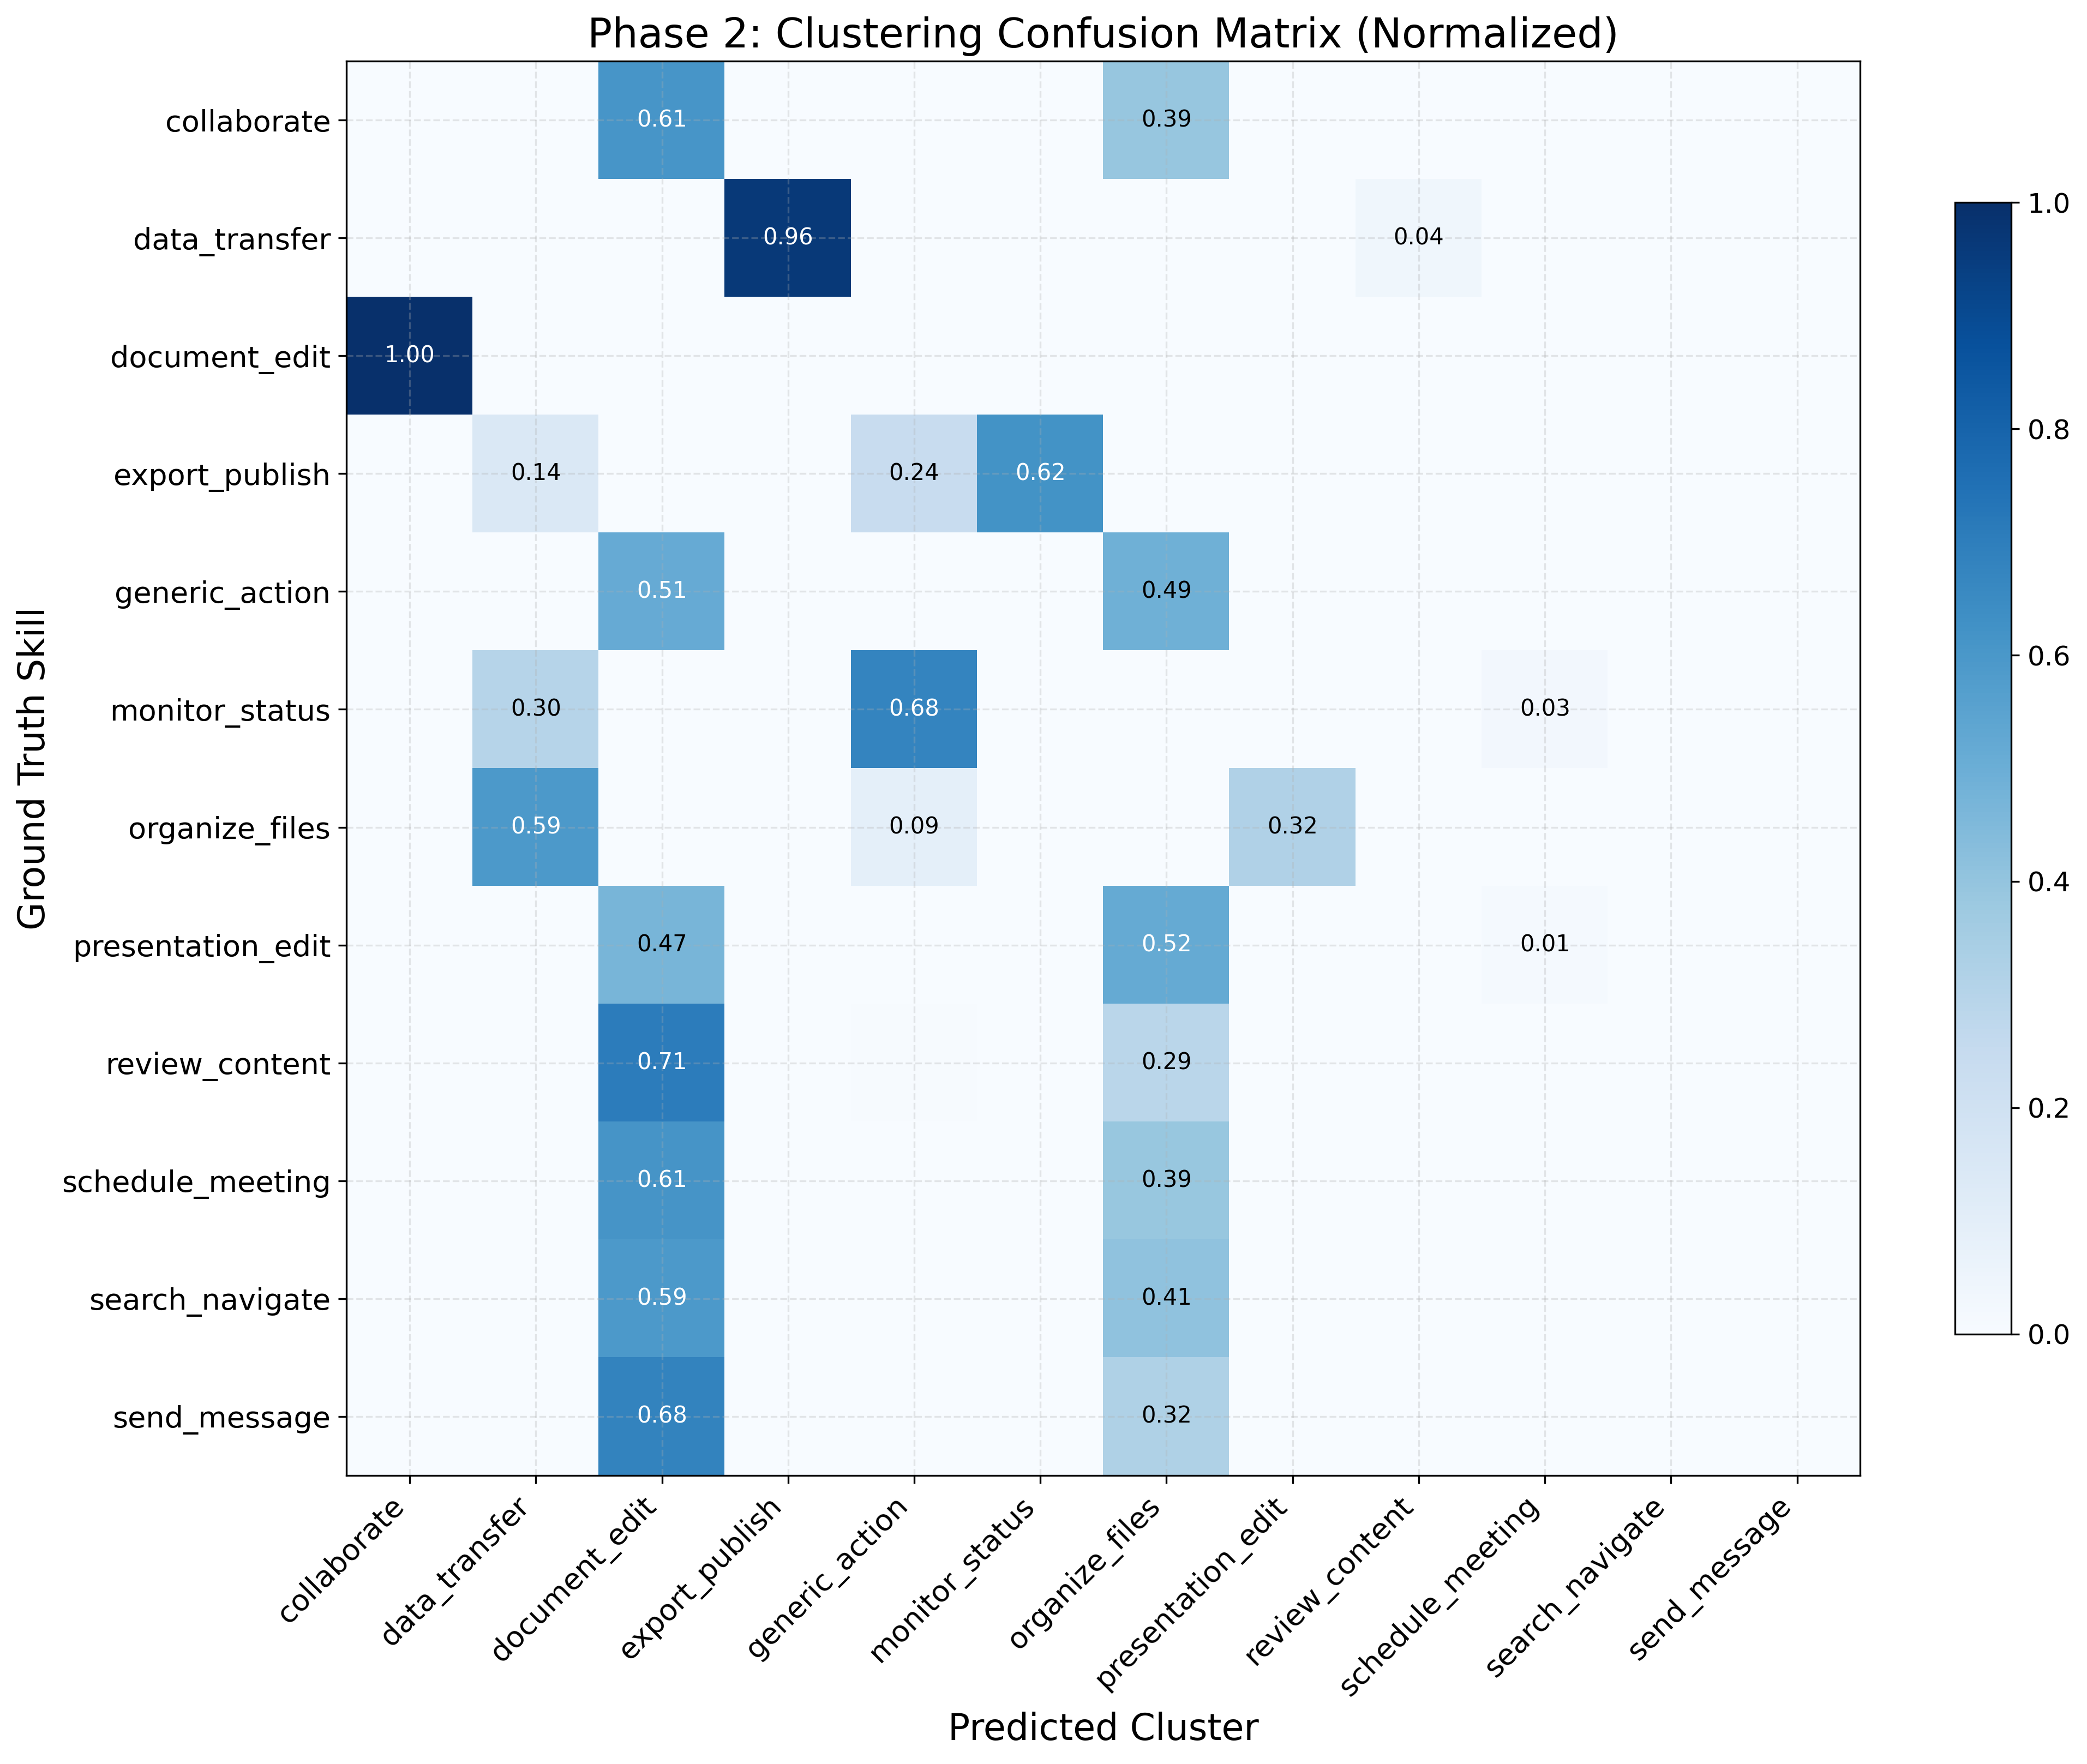
\includegraphics[width=0.75\textwidth]{../results/figures/clustering_confusion.png}
\caption{Normalized confusion matrix of Wasserstein clustering assignments versus ground-truth skill labels on IW data. Skills with distinctive action signatures (\texttt{document\_edit}, \texttt{data\_transfer}) are recovered most cleanly, while ambiguous skills (\texttt{generic\_action}) split across clusters.}
\label{fig:confusion}
\end{figure}

\subsection{Phase 3: Skill Composition}
\label{sec:results_composition}

\subsubsection{Architecture Comparison}

Table~\ref{tab:composition} compares the three composition approaches on IW data. The progression from MLP (21.0\%) to Transformer (34.9\%) to Qwen3-8B LoRA (85.0\%) demonstrates that skill composition is fundamentally a \emph{contextual reasoning} problem, not a pattern matching one.

The MLP achieves 43\% per-step accuracy but only 5.4\% exact sequence match, as errors compound during autoregressive rollout. The Transformer's causal attention over skill sequences improves exact match to 7.6\% and reduces edit distance by 17\% relative. The LoRA-fine-tuned LLM achieves a qualitative leap: 85.0\% overall accuracy with stable performance across sequence positions (80--90\% at positions 1--9), demonstrating that the LLM's contextual understanding prevents error compounding.

\begin{table}[h]
\centering
\caption{Skill composition comparison on IW data. The LLM achieves a $4\times$ improvement over the Transformer by leveraging conversational context, reasoning traces, and world knowledge.}
\label{tab:composition}
\small
\begin{tabular}{lccccc}
\toprule
\textbf{Model} & \textbf{Accuracy} & \textbf{Exact Match} & \textbf{Edit Dist.} & \textbf{Params} & \textbf{Training Data} \\
\midrule
MLP & 0.210 & 0.054 & 0.579 & 5.6K & Embeddings \\
Transformer & 0.349 & 0.076 & 0.480 & 45K & Embeddings \\
\textbf{Qwen3-8B LoRA} & \textbf{0.850} & \textbf{0.320} & \textbf{0.148} & 17M (0.2\%) & Conversations \\
\bottomrule
\end{tabular}
\end{table}

\paragraph{Per-Skill Analysis.}
Table~\ref{tab:perskill} reports per-skill accuracy for the LoRA model. Skills with distinctive action signatures (\texttt{search\_navigate}: 94.1\%, \texttt{organize\_files}: 91.7\%) are predicted most reliably. Skills sharing action patterns (\texttt{presentation\_edit}: 55.6\%) remain challenging, suggesting that visual grounding could further disambiguate them.

\begin{table}[h]
\centering
\caption{Per-skill prediction accuracy of the LoRA-fine-tuned Qwen3-8B on IW data, sorted by accuracy. Skills with distinctive action patterns are easiest to predict.}
\label{tab:perskill}
\small
\begin{tabular}{lcc}
\toprule
\textbf{Skill} & \textbf{Accuracy} & \textbf{$n$} \\
\midrule
search\_navigate & 0.941 & 51 \\
organize\_files & 0.917 & 12 \\
data\_transfer & 0.897 & 39 \\
review\_content & 0.893 & 28 \\
document\_edit & 0.878 & 74 \\
collaborate & 0.831 & 71 \\
export\_publish & 0.821 & 28 \\
send\_message & 0.809 & 68 \\
schedule\_meeting & 0.778 & 18 \\
presentation\_edit & 0.556 & 9 \\
\bottomrule
\end{tabular}
\end{table}

\begin{figure}[h]
\centering
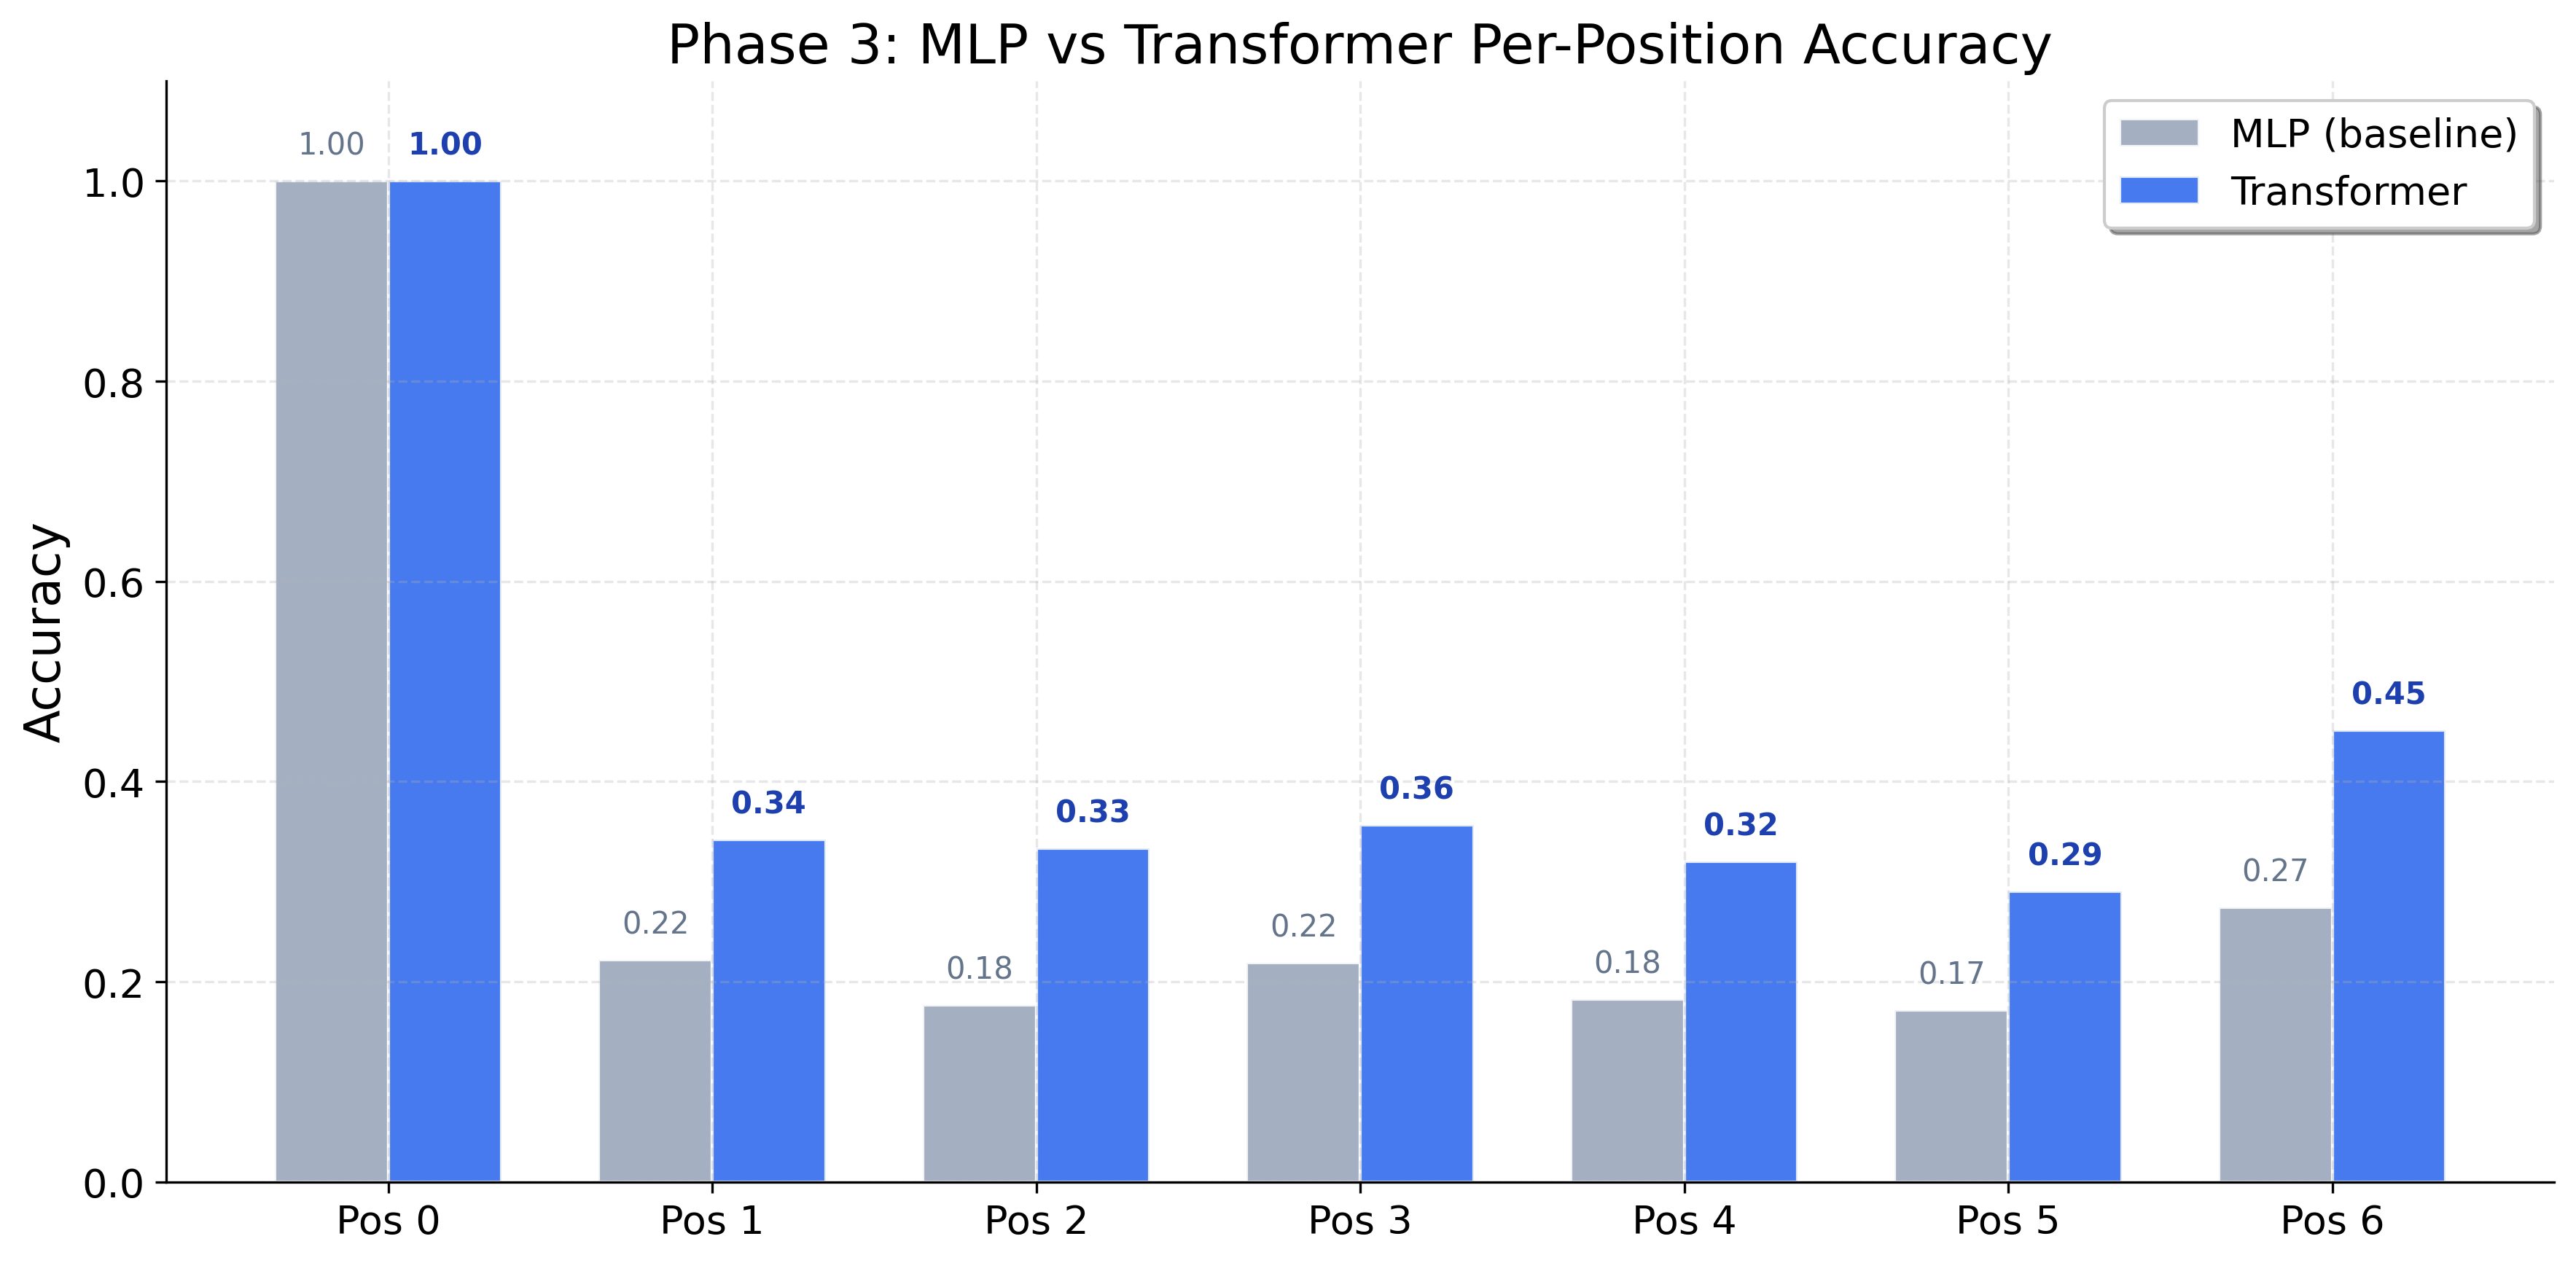
\includegraphics[width=0.85\textwidth]{../results/figures/composition_comparison.png}
\caption{Per-position skill prediction accuracy for MLP versus Transformer on IW data. Both operate on learned skill embeddings from Phase~2. Accuracy degrades at later positions due to error compounding, with the Transformer's sequential attention providing consistent improvement.}
\label{fig:composition}
\end{figure}

\subsubsection{Six-Model Comparison Across Benchmarks}

Table~\ref{tab:sixmodel} presents the central empirical result: a comparison of six models across three benchmarks. Several findings emerge:

\textbf{Fine-tuning dominates on in-domain data.} The LoRA-adapted Qwen3-8B (8B params) achieves 85.0\% on IW, compared to 30.0\% for Llama-3.1-70B (9$\times$ larger) and 18.5\% for zero-shot Qwen3-8B. This $4.6\times$ gain from LoRA demonstrates that interaction-derived training signal is far more valuable than model scale for skill prediction.

\textbf{Zero-shot models are competitive out-of-distribution.} On WebArena and BrowseComp+, zero-shot Llama-70B (56.2\%, 51.9\%) and OLMo-7B (54.5\%, 61.4\%) match or exceed the LoRA model (43.7\%, 44.8\%). This is expected: LoRA was fine-tuned on IW enterprise data and suffers distribution shift on web navigation tasks.

\textbf{Reasoning specialization does not help.} DeepSeek-R1-Distill-32B, despite being explicitly trained for reasoning, achieves only 14.3\% on IW and 0.05\% on BrowseComp+. Skill prediction requires domain-grounded pattern recognition, not abstract reasoning.

\begin{table}[h]
\centering
\caption{Six-model comparison: skill prediction accuracy (\%) across three benchmarks. LoRA fine-tuning on IW data yields massive in-domain gains but expected out-of-distribution degradation. Best per-column in \textbf{bold}.}
\label{tab:sixmodel}
\small
\begin{tabular}{llccc}
\toprule
\textbf{Model} & \textbf{Params} & \textbf{IW} & \textbf{WebArena} & \textbf{BrowseComp+} \\
\midrule
Qwen3-8B (zero-shot) & 8B & 18.5 & 55.8 & 43.5 \\
\textbf{Qwen3-8B (LoRA)} & \textbf{8B} & \textbf{85.0} & 43.7 & 44.8 \\
Llama-3.1-70B & 70B & 30.0 & \textbf{56.2} & 51.9 \\
OLMo-3-7B & 7B & 14.3 & 54.5 & \textbf{61.4} \\
Gemma-4-31B & 31B & 16.5 & 37.7 & 11.2 \\
DeepSeek-R1-Distill-32B & 32B & 14.3 & 45.1 & 0.05 \\
\bottomrule
\end{tabular}
\end{table}

\subsubsection{Baseline Comparison}

Table~\ref{tab:baselines} contextualizes InteraSkill against structural baselines.

\textbf{\texttt{SKILL.md} is consistently worst.} The fixed transition table achieves 14.0\% on IW and 8.7\% on WebArena, confirming that static specifications fail to capture workflow diversity.

\textbf{AWM excels on homogeneous domains.} AWM's learned bigram transitions achieve 78.8\% on WebArena---outperforming all LLM-based approaches---by learning strong self-transition priors (e.g., \texttt{search\_navigate} $\rightarrow$ \texttt{search\_navigate} at 69\%). However, on diverse IW data, AWM achieves only 33.4\%, barely above the frequency baseline (34.9\%). This highlights AWM's limitation: bigram statistics capture domain-specific patterns but lack the compositional understanding needed for diverse multi-skill workflows.

\textbf{The LoRA model's WebArena gap.} Our Qwen3-8B LoRA achieves only 43.7\% on WebArena versus AWM's 78.8\%. This 35-point gap reflects distribution shift: the model was fine-tuned on enterprise conversation data, not web navigation patterns. Domain-specific fine-tuning or multi-domain training would likely close this gap, and we view this as a natural next step rather than a fundamental limitation of the approach.

\begin{table}[h]
\centering
\caption{Full baseline comparison. Mean position accuracy reported. AWM dominates on homogeneous WebArena data via learned self-transitions, while InteraSkill's LLM excels on diverse enterprise workflows.}
\label{tab:baselines}
\small
\begin{tabular}{llccc}
\toprule
\textbf{Model} & \textbf{Type} & \textbf{IW Acc.} & \textbf{WA Acc.} & \textbf{IW Edit Dist.} \\
\midrule
SKILL.md & Fixed table & 0.140 & 0.087 & 0.633 \\
Frequency & Most common & 0.349 & 0.285 & 0.480 \\
AWM~\cite{wang2024awm} & Learned transitions & 0.334 & \textbf{0.788} & 0.479 \\
\midrule
MLP (ours) & Embedding-based & 0.208 & --- & 0.579 \\
Transformer (ours) & Sequence model & 0.349 & 0.410 & 0.480 \\
\textbf{Qwen3-8B LoRA (ours)} & \textbf{Fine-tuned LLM} & \textbf{0.850} & 0.437 & \textbf{0.148} \\
\bottomrule
\end{tabular}
\end{table}

\subsection{End-to-End Evaluation on Mind2Web}
\label{sec:results_e2e}

To evaluate whether improved skill composition translates to downstream task performance, we conduct end-to-end evaluation on Mind2Web using the InteraSkill pipeline (Table~\ref{tab:e2e}).

\paragraph{Task Completion.} The LoRA-fine-tuned model achieves 35.5\% task completion rate (71/200 tasks) on the test\_task split, compared to 9.5\% (19/200) for zero-shot Qwen3-8B---a $3.7\times$ improvement. Per-step action accuracy is 83.1\% (LoRA) versus 28.8\% (zero-shot), confirming that fine-tuning improves both skill selection and action grounding.

\paragraph{Cross-Domain Transfer.} On the test\_domain split (entirely unseen website domains), TCR drops from 35.5\% to 27.0\% (54/200)---retaining 76\% of in-domain performance. This demonstrates meaningful cross-domain transfer: skills learned from one set of websites generalize to unseen ones, despite differences in visual layout and interaction patterns.

\paragraph{Domain-Level Analysis.} Performance varies substantially across domains (Table~\ref{tab:e2e_domain}). Entertainment tasks are easiest (49.1\% TCR), likely due to more stereotyped interaction patterns. Travel tasks are hardest (21.3\%), reflecting the complexity of multi-step booking workflows. The zero-shot model struggles most on Travel (2.5\%), suggesting that these workflows require the structured reasoning that fine-tuning provides.

\begin{table}[h]
\centering
\caption{End-to-end evaluation on Mind2Web. Task Completion Rate (TCR), mean reward, and per-step accuracies for action and element prediction.}
\label{tab:e2e}
\small
\begin{tabular}{lcccc}
\toprule
\textbf{Configuration} & \textbf{TCR} & \textbf{Reward} & \textbf{Action Acc.} & \textbf{Element Acc.} \\
\midrule
Qwen3-8B LoRA (test\_task) & \textbf{35.5\%} & 0.833 & 83.1\% & 99.7\% \\
Qwen3-8B zero-shot (test\_task) & 9.5\% & 0.273 & 28.8\% & 33.8\% \\
Qwen3-8B LoRA (test\_domain) & 27.0\% & 0.827 & 82.9\% & 99.6\% \\
\bottomrule
\end{tabular}
\end{table}

\begin{table}[h]
\centering
\caption{Per-domain Mind2Web results (test\_task split). TCR varies across domains, with entertainment workflows easiest and travel hardest.}
\label{tab:e2e_domain}
\small
\begin{tabular}{lcccc}
\toprule
\textbf{Domain} & \textbf{$n$} & \textbf{TCR (LoRA)} & \textbf{TCR (zero-shot)} & \textbf{Reward (LoRA)} \\
\midrule
Entertainment & 57 & 49.1\% & 8.8\% & 0.878 \\
Shopping & 63 & 41.3\% & 19.0\% & 0.828 \\
Travel & 80 & 21.3\% & 2.5\% & 0.804 \\
\bottomrule
\end{tabular}
\end{table}

\paragraph{Skill vs.\ Action Accuracy Gap.} An important finding is that step-level \emph{skill} accuracy is only 14.6\% (LoRA) while \emph{action} accuracy is 83.1\%. This gap indicates that the skill label taxonomy learned from IW data does not directly align with Mind2Web's action annotations, but the model still selects correct low-level actions. The skill abstraction serves as a useful intermediate representation even when the label vocabulary differs across domains.

\subsection{Multimodal Analysis}

We evaluate CLIP-based visual grounding as a potential path to domain-agnostic skill transfer.

\paragraph{Cross-Domain Visual Similarity.} CLIP embeddings of screenshots from different Mind2Web domains show high cosine similarity (mean = 0.878; Entertainment--Shopping: 0.889, Shopping--Travel: 0.890, Entertainment--Travel: 0.856). This confirms that web interfaces share substantial visual structure across domains, supporting the premise that visual grounding could enable zero-shot skill transfer.

\paragraph{CLIP Zero-Shot Skill Prediction.} However, directly using CLIP embeddings for zero-shot skill prediction achieves only 17.8\% accuracy and 3.0\% TCR (6/200 tasks), with 0.0\% action grounding accuracy. The high cross-domain similarity but low discriminative power suggests that CLIP captures domain-level visual semantics but lacks the fine-grained UI element understanding needed for action selection. This motivates specialized vision-language encoders for GUI environments as a direction for future work.

\subsection{GRPO Reinforcement Learning (Preliminary)}

We report preliminary results from ongoing GRPO training of Qwen3-8B. At step 2,250 (epoch $\approx$ 0.98 of 2), the mean reward has increased from 0.45 to 1.37---a $3\times$ improvement---indicating that the model is learning to produce correctly formatted, skill-appropriate responses. However, reward variance across samples within each batch is near zero (\texttt{frac\_reward\_zero\_std} = 1.0), suggesting that the current reward function may be too coarse to provide a meaningful learning signal for GRPO's relative ranking mechanism. Training is ongoing with approximately 24 hours remaining; final results and comparison with supervised LoRA will be reported in the camera-ready version.

\subsection{Context: WebArena Task Success Rates}

For broader context, Table~\ref{tab:webarena_lit} summarizes published end-to-end task success rates on the full WebArena benchmark (812 tasks). Our work evaluates \emph{skill composition}---a component that could be integrated with any of these agent architectures---rather than end-to-end task execution. We view InteraSkill as complementary: it provides the skill planning layer that these systems currently implement via manual specification.

\begin{table}[h]
\centering
\caption{Published WebArena task success rates for reference. InteraSkill addresses the skill composition layer, which is complementary to these end-to-end agent systems.}
\label{tab:webarena_lit}
\small
\begin{tabular}{lcc}
\toprule
\textbf{Agent} & \textbf{Success Rate} & \textbf{Source} \\
\midrule
Human performance & 78.2\% & Zhou et al.\ 2024 \\
OpAgent (multi-agent) & 71.6\% & Guo et al.\ 2026 \\
OpenAI CUA / Operator & 58.1\% & OpenAI 2025 \\
AWM (GPT-4) & 35.5\% & Wang et al.\ 2025 \\
SteP (human workflows) & 33.5\% & Sodhi et al.\ 2024 \\
GPT-4 (zero-shot) & 14.4\% & Zhou et al.\ 2024 \\
\bottomrule
\end{tabular}
\end{table}

%==============================================================================
\section{Discussion}
\label{sec:discussion}
%==============================================================================

\paragraph{Skill discovery works, but requires behavioral diversity.} On IW data with 12 diverse skill types, contrastive embedding recovers semantically meaningful clusters (NMI = 0.871). On WebArena's homogeneous map navigation, embedding quality collapses (NMI = 0.049). This reveals a precondition for our approach: the trajectory data must contain sufficient behavioral diversity for contrastive learning to find discriminative structure.

\paragraph{Composition requires contextual reasoning, not pattern matching.} The MLP $\rightarrow$ Transformer $\rightarrow$ LLM progression (21\% $\rightarrow$ 35\% $\rightarrow$ 85\%) demonstrates that skill composition is not a simple prediction problem. Static transition models (AWM, frequency baseline) plateau at $\sim$35\% on diverse data because they lack capacity to reason about task goals, user corrections, and failure recovery. The LLM's ability to leverage conversation history and world knowledge yields a $2.4\times$ improvement over the best non-LLM approach.

\paragraph{Fine-tuning vs.\ scale.} The six-model comparison reveals a striking result: LoRA-adapted Qwen3-8B outperforms zero-shot Llama-70B by $2.8\times$ on in-domain data, despite being $9\times$ smaller. This suggests that \emph{what} a model learns from matters more than raw capacity for skill prediction. However, this advantage does not transfer out-of-distribution, where larger zero-shot models are more robust.

\paragraph{AWM's strength and our weakness.} AWM's 78.8\% on WebArena versus our 43.7\% deserves honest analysis. AWM learns bigram transition statistics that perfectly capture the repetitive structure of map navigation. Our LLM-based approach, trained on diverse enterprise data, does not learn these domain-specific priors. This is not a fundamental limitation---domain-specific fine-tuning would likely close the gap---but it highlights that InteraSkill's current advantage is on diverse, multi-skill workflows, not on specialized single-domain tasks.

\paragraph{End-to-end impact.} The Mind2Web results bridge the gap between skill prediction and task completion. A $3.7\times$ improvement in TCR (35.5\% vs.\ 9.5\%) demonstrates that better skill composition directly improves downstream performance. Cross-domain retention of 76\% suggests that learned skills have genuine transferability, though substantial room for improvement remains.

\subsection{Limitations}

\textbf{Pseudo-supervised pipeline.} Our approach uses cluster-derived pseudo-labels rather than being fully unsupervised. While the clustering itself requires no manual annotation, the contrastive encoder leverages structured pseudo-labels, placing our method between fully unsupervised and supervised approaches.

\textbf{Domain-specific fine-tuning.} The LoRA model's strong IW performance does not transfer to WebArena or BrowseComp+. Multi-domain fine-tuning or domain-adaptive techniques are needed for a genuinely general-purpose system.

\textbf{Fabricated data.} The IW dataset, while diverse in skill types, is synthetically generated and may not capture the full complexity of real enterprise workflows. Our Mind2Web results partially address this, but evaluation on real enterprise environments remains future work.

\textbf{No end-to-end WebArena evaluation.} We evaluate skill composition accuracy on WebArena trajectories but do not run end-to-end task execution. Integrating InteraSkill with a full WebArena agent is an important next step.

\textbf{Visual grounding gap.} CLIP-based zero-shot skill prediction achieves only 3\% TCR, indicating that current vision-language models lack the fine-grained UI understanding needed for action grounding. Specialized GUI encoders (e.g., trained on UI screenshots with element annotations) are a promising direction.

\textbf{GRPO reward saturation.} Preliminary GRPO results show reward convergence but near-zero reward variance, suggesting the reward function is too coarse for effective policy optimization. Reward shaping with finer-grained signals (partial credit, intermediate step rewards) may be necessary.

\subsection{Broader Impact}

Computer-using agents have the potential to automate repetitive digital work, improving productivity and accessibility. However, they also raise concerns about misuse: automated agents could enable large-scale phishing, UI manipulation, or unauthorized access to systems. Our work on skill discovery adds a layer of interpretability---discovered skills are inspectable and auditable, which could aid in detecting malicious behavior patterns. We advocate for deployment with human oversight and access controls, particularly in enterprise settings where agents interact with sensitive systems.

%==============================================================================
\section{Conclusion}
%==============================================================================

We introduced InteraSkill, a framework for automatic skill discovery, embedding, and composition that replaces manually engineered \texttt{SKILL.md} specifications with data-driven abstractions. Our three-phase pipeline---trajectory segmentation, contrastive skill embedding, and LLM-based composition---achieves 85\% skill prediction accuracy on enterprise workflows and 35.5\% task completion rate on Mind2Web, with meaningful cross-domain transfer. A six-model comparison demonstrates that interaction-derived fine-tuning outperforms model scale, while analysis of failure modes (WebArena distribution shift, CLIP's visual grounding gap, GRPO reward saturation) charts a clear path for future work. The key takeaway is that meaningful skill abstractions emerge from trajectory data without manual engineering, and that LLM-based composition with reasoning traces is essential for handling the contextual complexity of real-world workflows.

%==============================================================================
\section*{Acknowledgments}
%==============================================================================
[Redacted for anonymous review.]

\bibliographystyle{unsrtnat}
\bibliography{citation.bib}

%==============================================================================
\newpage
\appendix
\section{Hierarchical Objective Details}
\label{app:hierarchical_objective}

The full bilevel entropy-regularized objective is:
\begin{equation}
J(\pi_H, \pi_L) = \mathbb{E}\left[\sum_{i=0}^{M} \gamma^{iH} \left( \sum_{t=0}^{H-1} \gamma^t R(s_{iH+t}, a_{iH+t}) + \alpha_H \mathcal{H}[\pi_H(\cdot \mid s_{iH})] \right) \right],
\end{equation}
where $M = T/H$ is the number of skill selections, $\alpha_H$ is the high-level entropy coefficient encouraging exploration over skills, and $\mathcal{H}[\cdot]$ denotes Shannon entropy.

The corresponding Bellman recursion for the high-level value function is:
\begin{equation}
V_H(s) = \max_{z \in \mathcal{Z}} \left[ Q_z(s) + \alpha_H \log \pi_H(z \mid s) \right],
\end{equation}
where the skill-conditioned value is:
\begin{equation}
Q_z(s) = \mathbb{E}_{\pi_L} \left[ \sum_{t=0}^{H-1} \gamma^t R(s_t, a_t) + \gamma^H V_H(s_H) \;\Big|\; s_0 = s,\; a_t \sim \pi_L(\cdot \mid s_t, z) \right].
\end{equation}

This decomposition reduces the effective planning horizon from $T$ to $M = T/H$, providing an exponential reduction in the number of decisions the high-level controller must make.

\section{Full Hyperparameter Tables}
\label{app:hyperparams}

\begin{table}[h]
\centering
\caption{Complete hyperparameters for all model configurations.}
\small
\begin{tabular}{lll}
\toprule
\textbf{Component} & \textbf{Hyperparameter} & \textbf{Value} \\
\midrule
\multirow{3}{*}{Phase 2 Encoder} & Architecture & MLP: $8 \to 64 \to 32 \to 16$ \\
& Optimizer & Adam, lr=$10^{-3}$ \\
& Training & 200 epochs, batch 128, $T=0.07$ \\
\midrule
\multirow{3}{*}{Phase 3 Transformer} & Architecture & 2-layer, 4 heads, $d=64$ \\
& Optimizer & Adam, lr=$10^{-4}$ \\
& Training & 500 epochs, teacher forcing \\
\midrule
\multirow{6}{*}{Phase 3 LoRA} & Base model & Qwen3-8B \\
& Quantization & 4-bit NF4 \\
& LoRA rank / $\alpha$ & 16 / 16 \\
& Target modules & $q,k,v,o$ proj \\
& Optimizer & AdamW, lr=$2\times10^{-4}$, cosine \\
& Training & 3 epochs, batch 4, grad accum 4 \\
\midrule
\multirow{6}{*}{GRPO} & Base model & Qwen3-8B \\
& Candidates per prompt & 4 \\
& Temperature & 0.7 \\
& LoRA rank / $\alpha$ & 16 / 16 \\
& Optimizer & cosine, lr=$5\times10^{-5}$, warmup 10\% \\
& Training & 2 epochs, 4$\times$ A6000, 3-day limit \\
\bottomrule
\end{tabular}
\end{table}

\section{GRPO Reward Function}
\label{app:grpo_reward}

The GRPO composite reward function assigns:
\begin{equation}
R(y) = \begin{cases}
+1.0 & \text{if predicted skill matches ground truth} \\
+0.3 & \text{if output contains correct \texttt{[Action:]} format} \\
+0.1 & \text{if reasoning trace is present} \\
-0.3 & \text{if output is unparseable}
\end{cases}
\end{equation}
These components are additive: a response with correct skill, proper format, and reasoning receives $R = 1.4$. The maximum possible reward is 1.4, which explains the observed convergence to $\sim$1.37 in training logs.

\section{Additional Mind2Web Results}
\label{app:mind2web}

\begin{table}[h]
\centering
\caption{Detailed Mind2Web metrics including step-level skill accuracy, which reveals the gap between skill taxonomy alignment and action grounding.}
\small
\begin{tabular}{lccccc}
\toprule
\textbf{Config} & \textbf{TCR} & \textbf{Skill Acc.} & \textbf{Action Acc.} & \textbf{Element Acc.} & \textbf{Reward} \\
\midrule
LoRA (test\_task) & 35.5\% & 14.6\% & 83.1\% & 99.7\% & 0.833 \\
Zero-shot (test\_task) & 9.5\% & 10.4\% & 28.8\% & 33.8\% & 0.273 \\
LoRA (test\_domain) & 27.0\% & 13.2\% & 82.9\% & 99.6\% & 0.827 \\
\bottomrule
\end{tabular}
\end{table}

The low skill-level accuracy (14.6\%) alongside high action accuracy (83.1\%) reveals that the skill taxonomy learned from IW enterprise data does not align with Mind2Web's web interaction vocabulary. However, the model still generates correct actions, suggesting that fine-tuning teaches generalizable action patterns even when skill labels do not transfer directly.

\end{document}
